\documentclass[12pt, twoside]{book}
\usepackage[a4paper,top=2.5cm,bottom=2.5cm,left=3.5cm,right=2cm]{geometry}
\usepackage[utf8]{inputenc}
\usepackage[T1]{fontenc}
\usepackage{graphicx}
\usepackage{url}
\usepackage[hidelinks,breaklinks]{hyperref}
\usepackage[slovak]{babel} % vypnite pre prace v anglictine
\linespread{1.25} % hodnota 1.25 by mala zodpovedat 1.5 riadkovaniu

%\usepackage{fancyhdr}
\usepackage{amsmath}
\usepackage{float}
\usepackage{amsthm}
\usepackage{amsmath}
\usepackage{amsfonts}
\usepackage{xfrac}
\usepackage{caption}
\usepackage{subcaption}
\usepackage{gensymb}
\usepackage{enumitem}

\usepackage{pgfplots}
\pgfplotsset{compat=1.18, width=10cm}

\newtheorem{definition}{Definícia}[chapter]
\newtheorem{theorem}{Veta}[chapter]
\newtheorem{lemma}{Lema}[chapter]

\theoremstyle{definition}
\newtheorem{corollary}{Dôsledok}[chapter]
\newtheorem{note}{Poznámka}
\newtheorem{example}{Príklad}

%euler, pxtx, cm
\usepackage[scr=dutchcal,
scrscaled=1.1]{mathalpha}

% -------------------
% --- Definicia zakladnych pojmov
% --- Vyplnte podla vasho zadania
% -------------------
\def\mfrok{2024}
\def\mfnazov{Obálka systému plôch}
\def\mftyp{Diplomová práca}
\def\mfautor{Bc. Jana Tutková}
\def\mfskolitel{doc. RNDr. Pavel Chalmovianský, PhD. }

%ak mate konzultanta, odkomentujte aj jeho meno na titulnom liste
\def\mfkonzultant{tit. Meno Priezvisko, tit. }  

\def\mfmiesto{Bratislava, \mfrok}

%aj cislo odboru je povinne a je podla studijneho odboru autora prace
\def\mfodbor{1113 Matematika} 
\def\program{ Počítačová grafika a geometria }
\def\mfpracovisko{ Katedra algebry a geometrie }
\begin{document}     
\frontmatter


% -------------------
% --- Obalka ------
% -------------------
\thispagestyle{empty}

\begin{center}
\sc\large
Univerzita Komenského v Bratislave\\
Fakulta matematiky, fyziky a informatiky

\vfill

{\LARGE\mfnazov}\\
\mftyp
\end{center}

\vfill

{\sc\large 
\noindent \mfrok \hfill
\mfautor
}

\eject % EOP i
% --- koniec obalky ----

% -------------------
% --- Titulný list
% -------------------

\thispagestyle{empty}
\noindent

\begin{center}
\sc  
\large
Univerzita Komenského v Bratislave\\
Fakulta matematiky, fyziky a informatiky

\vfill

{\LARGE\mfnazov}\\
\mftyp
\end{center}

\vfill

\noindent
\begin{tabular}{ll}
Študijný program: & \program \\
Študijný odbor: & \mfodbor \\
Školiace pracovisko: & \mfpracovisko \\
Školiteľ: & \mfskolitel \\
% Konzultant: & \mfkonzultant \\
\end{tabular}

\vfill


\noindent \mfmiesto\\
\mfautor

\eject % EOP i


% --- Koniec titulnej strany


% -------------------
% --- Zadanie z AIS
% -------------------
% v tlačenej verzii s podpismi zainteresovaných osôb.
% v elektronickej verzii sa zverejňuje zadanie bez podpisov

\newpage 
\thispagestyle{empty}
\hspace{-2cm}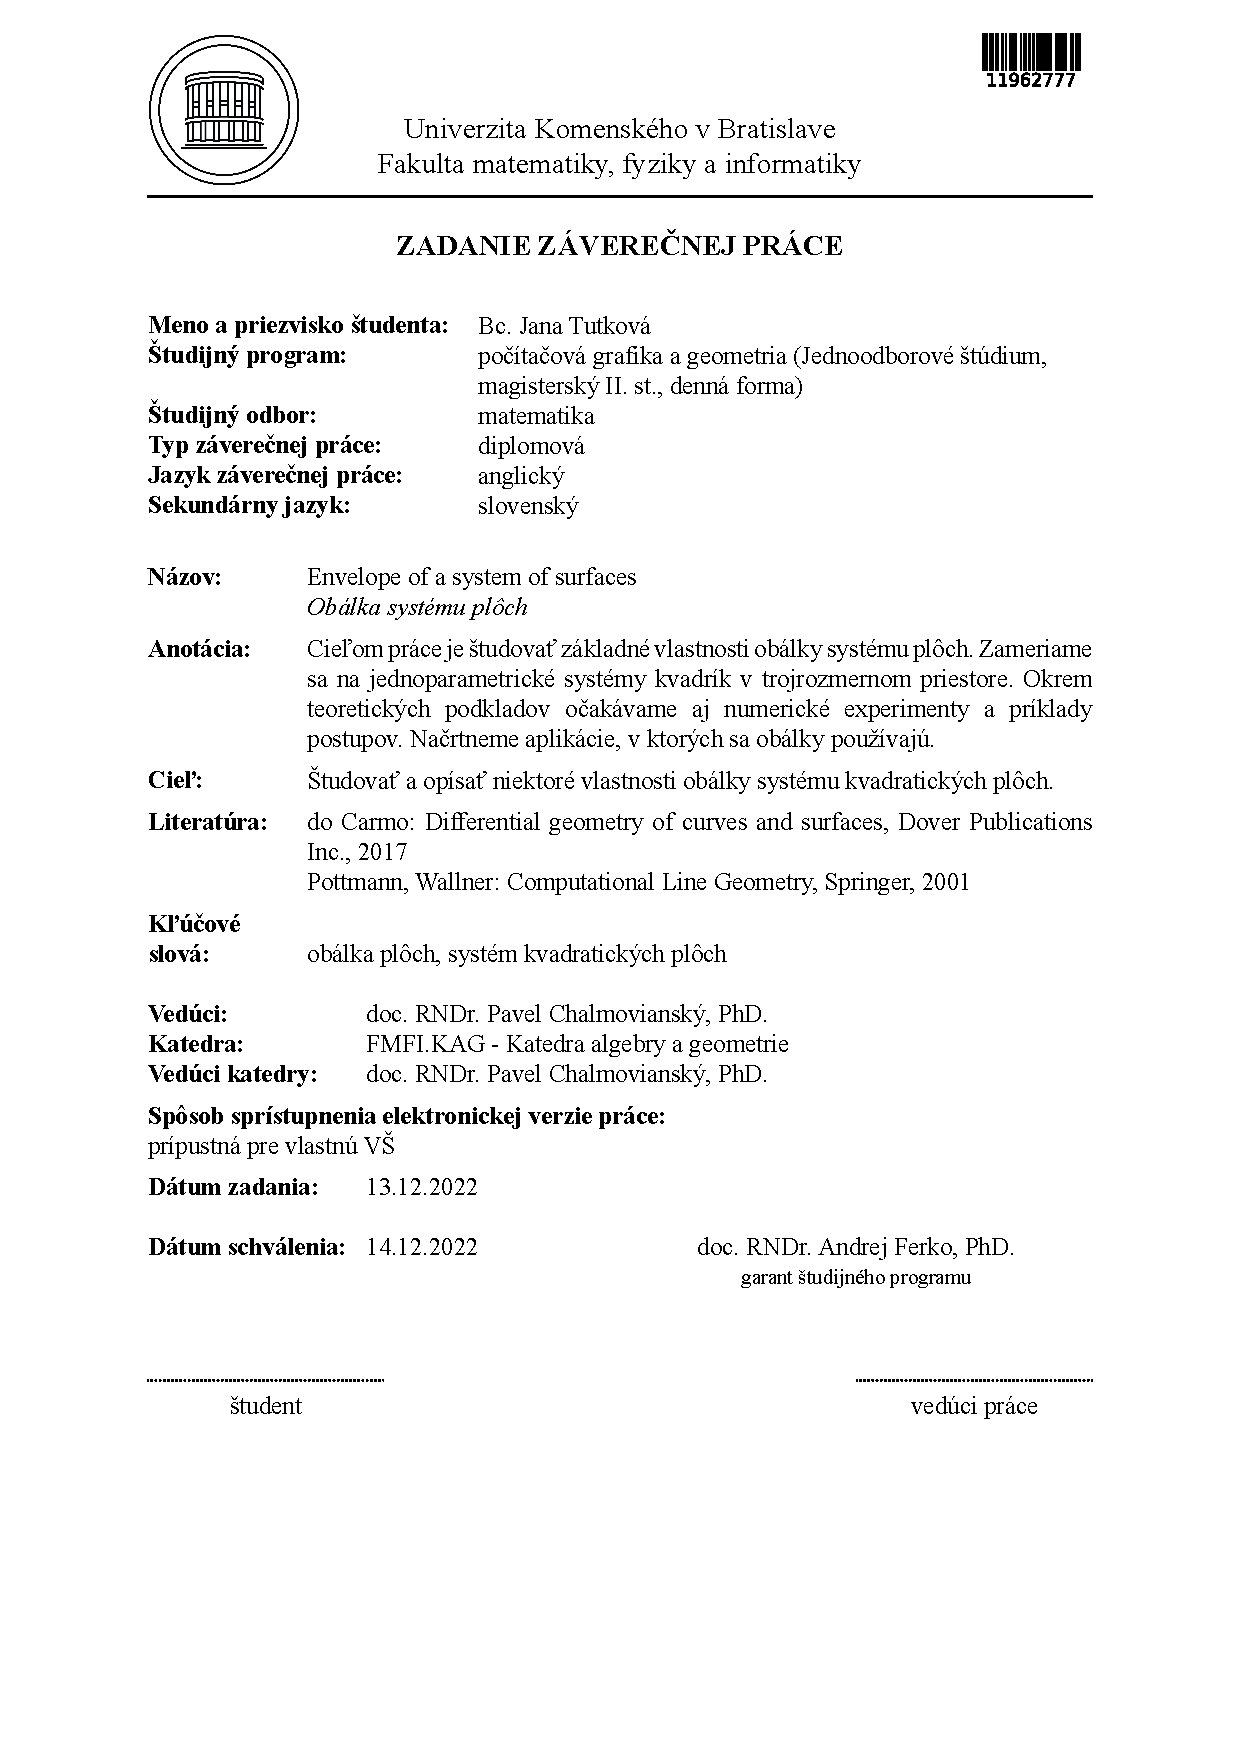
\includegraphics[width=1.1\textwidth]{images/zadanieJT.pdf}

% --- Koniec zadania

\frontmatter

% -------------------
%   Poďakovanie - nepovinné
% -------------------
\setcounter{page}{3}
\newpage 
~

\vfill
{\bf Poďakovanie:}

% --- Koniec poďakovania

% -------------------
%   Abstrakt - Slovensky
% -------------------
\newpage 
\section*{Abstrakt}
Tutková, Jana: Obálka systému plôch. Diplomová práca, Univerzita Komenského. Fakulta matematiky, fyziky a informatiky; Katedra algebry a geometrie. Bratislava: FMFI UK, 2023.


\paragraph*{Kľúčové slová:} obálka plôch, systém kvadratických plôch
% --- Koniec Abstrakt - Slovensky


% -------------------
% --- Abstrakt - Anglicky 
% -------------------
\newpage 
\section*{Abstract}
Tutková, Jana: Envelope of a system of surfaces. Master's  thesis, Comenius University. Faculty of Mathematics, Physics and Informatics; Department of algebra and geometry. Bratislava: FMFI UK, 2023.



\paragraph*{Keywords:} envelope of surfaces, system of quadratic surfaces

% --- Koniec Abstrakt - Anglicky

% -------------------
% --- Predhovor - v informatike sa zvacsa nepouziva
% -------------------
%\newpage 
%\thispagestyle{empty}
%
%\huge{Predhovor}
%\normalsize
%\newline
%Predhovor je všeobecná informácia o práci, obsahuje hlavnú charakteristiku práce 
%a okolnosti jej vzniku. Autor zdôvodní výber témy, stručne informuje o cieľoch 
%a význame práce, spomenie domáci a zahraničný kontext, komu je práca určená, 
%použité metódy, stav poznania; autor stručne charakterizuje svoj prístup a svoje 
%hľadisko. 
%
% --- Koniec Predhovor


% -------------------
% --- Obsah
% -------------------

\newpage 

\tableofcontents

% ---  Koniec Obsahu

% -------------------
% --- Zoznamy tabuliek, obrázkov - nepovinne
% -------------------

\newpage 

\listoffigures
\listoftables

% ---  Koniec Zoznamov

\mainmatter


\input uvod.tex 

\input kapitola.tex

\input numerika.tex

\input obalka_sfer.tex

\input implementacia.tex

\input vysledky_prace.tex

\input zaver.tex

% -------------------
% --- Bibliografia
% -------------------


\newpage	

\backmatter

\thispagestyle{empty}
\nocite{*}
\clearpage

\bibliographystyle{plain}
\bibliography{literatura} 

%Prípadne môžete napísať literatúru priamo tu
\begin{thebibliography}{99}

\bibitem{Bab00} Babušíková J., Slodička M., Weisz J. 2000. \textit{Numerické metódy.} Univerzita Komenského v Bratislave. ISBN 80-223-1384-X. Dostupné na internete: \url{http://hore.dnom.fmph.uniba.sk/~babusikova/skripta.pdf}.

\bibitem{Blender} Blender documentation: Blender 4.0 Reference Manual. Dostupné na internete: \url{https://docs.blender.org/manual/en/latest/index.html}.

\bibitem{BlenderAPI} Blender documentation: Blender 4.0 Python API Documentation. Dostupné na internete: \url{https://docs.blender.org/api/current/}.

\bibitem{BlenderMesh} Blender documentation: Mesh Operator. Dostupné na internete: \url{https://docs.blender.org/api/current/bpy.ops.mesh.html}.

\bibitem{BlenderContext} Blender documentation: Context Access. Dostupné na internete: \url{https://docs.blender.org/api/current/bpy.context.html}.

\bibitem{BlenderDownload} Blender download. Dostupné na internete:\url{https://www.blender.org/download/}.

\bibitem{Bien16} Biernet A. 2016. Visualisierung und grafische Anwendung von Kanalflächen. Martin-Luther-Universität Halle-Wittenberg, Naturwissenschaftliche Fakultät III. Halle (Saale). Dissertation. Dostupné na internete: \url{https://digital.bibliothek.uni-halle.de/hs/content/titleinfo/2416652}.

\bibitem{Bru81} Bruce, J. W., Giblin, P. J. 1981. What Is an Envelope? \textit{The Mathematical Gazette}, 65(433), 186-192. Dostupné na internete: \url{http://www.jstor.org/stable/3617131}.

\bibitem{doCarmo17} do Carmo M. P. 2017. \textit{Differential Geometry of Curves and Surfaces}, New York. Dover Publications Inc., Mineola. ISBN-13: 978-0-486-80699-0.

\bibitem{Gro97} Grossfield, A. 1997. What Are Differential Equations: A Review Of Curve Families. Paper presented at 1997 Annual Conference, Milwaukee, Wisconsin. 10.18260/1-2--6898. Dostupné na internete: \url{https://216.185.13.174/what-are-differential-equations-a-review-of-curve-families}.

\bibitem{Hla} Hlavička R., Růžičková I. Numerické metody. Brno. Dostupné na internete: \url{http://physics.ujep.cz/ jskvor/NME/DalsiSkripta/Numerika.pdf}.

\bibitem{Chalm} Chalmovianská, J. Skriptá k predmetu Algebraická geometria. Dostupné na internete: \url{http://fractal.dam.fmph.uniba.sk/~pilnikova/ag1.html}.

\bibitem{Chud09} Chudinov P. 2009. Numerical-analytical Algorithm for Constructing the Envelope of the Projectile Trajectories in Midair. Dostupné na internete: \url{https://doi.org/10.48550/arXiv.0902.0520}.

\bibitem{Kar00} Karčiauskas K., Krasauskas R. 2000. Rational rolling ball blending of natural quadrics. \textit{Mathematical Modelling and Analysis,} Volume 5, Pages 97-107. Dostupné na internete: \url{https://www.researchgate.net/publication/233265253_Rational_rolling_ball_blending_of_natural_quadrics}.

\bibitem{Lee12} Lee, J. 2012. \textit{Introduction to Smooth Manifolds.} Graduate Texts in Mathematics. New York. Springer. 2. edition. Dostupné na internete: \url{https://doi.org/10.1007/978-1-4419-9982-5}.

\bibitem{Ode20} Odehnal B., Stachel H., Glaeser G. 2020. \textit{The Universe of Quadrics.} Vienna. Springer-Verlag. ISBN 978-3-662-61052-7. Dostupné na internete: \url{https://doi.org/10.1007/978-3-662-61053-4}.

\bibitem{Pet97} Peternell, M., Pottmann H. 1997. Computing Rational Parametrizations of Canal Surfaces. \textit{Journal of Symbolic Computation}, Volume 23, Issues 2–3, Pages 255-266, ISSN 0747-7171. Dostupné na internete: \url{https://doi.org/10.1006/jsco.1996.0087}.

\bibitem{Pet08} Peternell M., Odehnal B., Sampoli M. L.,
On quadratic two-parameter families of spheres and their envelopes, \textit{Computer Aided Geometric Design}, Volume 25, Issues 4–5, 2008, Pages 342-355, ISSN 0167-8396. Dostupné na internete: \url{https://doi.org/10.1016/j.cagd.2007.10.007}.

\bibitem{Pet98} Peternell M., Pottmann H. 1998. A Laguerre geometric approach to rational offsets, \textit{Computer Aided Geometric Design},
Volume 15, Issue 3, Pages 223-249, ISSN 0167-8396. Dostupné na internete: \url{https://doi.org/10.1016/S0167-8396(97)00024-1}.

\bibitem{Pott09} Pottmann H., Peternell M. 2009. Envelopes – Computational Theory and Applications. Proceedings of Spring Conference on Computer Graphics. Dostupné na internete: \url{https://www.geometrie.tuwien.ac.at/geom/ig/peternell/env.pdf}.

\bibitem{Pott98} Pottmann H., Peternell M. 1998. Applications of Laguerre geometry in CAGD. \textit{Computer Aided Geometric Design}, Volume 15, Issue 2, Pages 165-186, ISSN 0167-8396. Dostupné na internete: \url{https://doi.org/10.1016/S0167-8396(97)00023-X}.

\bibitem{Pott01} Pottmann, H., Wallner, J. 2001. \textit{Computational Line Geometry}. Springer-Verlag.

\bibitem{PythonDocumentation} Python documentation. Dostupné na internete: \url{https://docs.python.org/3/}.

\bibitem{Python} Python download. Dostupné na internete: \url{https://www.python.org/downloads}.

\bibitem{Skop20} Skopenkov M. et al. 2020. Characterizing envelopes of moving rotational cones and applications in CNC machining, \textit{Computer Aided Geometric Design}, Volume 83, 101944, ISSN 0167-8396. Dostupné na internete: \url{https://doi.org/10.1016/j.cagd.2020.101944}.

\bibitem{VSCode} Visual Studio Code download. Dostupné na internete:\url{https://code.visualstudio.com/download}.

\bibitem{Vra22} Vráblíková J. 2022. Envelopes of implicit surfaces. Mathematical Institute of Charles University. Prague. Master's thesis. Dostupné na internete: \url{https://dodo.is.cuni.cz/bitstream/handle/20.500.11956/171858/120411574.pdf?sequence=1&isAllowed=y}.

\bibitem{WebbBridge} Obrázok Webbov Most. Dostupné na internete: \url{http://www.yannarthusbertrand2.org/collection/australia/#mwl-3844}.

\bibitem{Rollingballblends} Obrázok Rolling ball blends. Dostupné na internete:  \url{https://www2.mathematik.tu-darmstadt.de/~ehartmann/pub/parblrb_abs/parblrb_abs.html}.

Všetky online zdroje boli dostupné dňa 10.05.2024.

%\bibitem{Bru92} Bruce, J., Giblin, P. (1992). Envelopes. In Curves and Singularities: A Geometrical Introduction to Singularity Theory (pp. 99-132). Cambridge: Cambridge University Press. doi:10.1017/CBO9781139172615.007


%\bibitem{Ber88} Berger, M., Gostiaux, B. (1988). Differential Geometry: Manifolds, Curves, and Surfaces. Graduate Texts in Mathematics, vol 115. Springer, New York, NY. %https://doi.org/10.1007/978-1-4612-1033-7_6
%nemam

%\bibitem{Kar78} Karger, A. Kinematic geometry of regular motions in homogeneous space. Czechoslovak Mathematical Journal, 28:327 – 338, 1978.

%Richard Morris. A client-server system for the visualisation of algebraic surfaces on the web. In Algebra, Geometry and Software Systems, pages 239–253. Springer, 2003.

%W. Kuhnel: Differential Geometry Curves-Surfaces-Manifolds
%dostupne online: https://books.google.sk/books/about/Differential_Geometry_Manifolds_Curves_a.html?id=SFXSBwAAQBAJ&redir_esc=y

%Spivak: A comprehensive introduction to Differential Geometry
%dostupné online: https://kupdf.net/download/michael-spivak-a-comprehensive-introduction-to-differential-geometry-vol-5_5afdb2c9e2b6f5cb4c79488b_pdf

\end{thebibliography}

%---koniec Referencii

% -------------------
%--- Prilohy---
% -------------------

%Nepovinná časť prílohy obsahuje materiály, ktoré neboli zaradené priamo  do textu. Každá príloha sa začína na novej strane.
%Zoznam príloh je súčasťou obsahu.

\newpage
%\addcontentsline{toc}{chapter}{Príloha A}
\input AppendixA.tex
%
%\addcontentsline{toc}{chapter}{Appendix B}
%\input AppendixB.tex

\end{document}






